\chapter{Perancangan}
\label{chap:perancangan}

Bab ini membahas tentang perancangan setiap fitur yang akan diimplementasi pada perangkat lunak Sharif Judge. 

\section{Mengganti method \textit{shell\_exec("rm ...")} menjadi unlink()}
Method \textit{shell\_exec("rm ...")} yang memiliki fungsi untuk menghapus sebuah file terdapat pada file controller Assignment.php tepatnya di baris kode 425 dan 473

Assignments.php
\begin{lstlisting}[basicstyle=\ttfamily, frame=single,
columns=fullflexible, keepspaces=true]

...
423	// Upload Tests (zip file)
424	
425	shell_exec('rm -f '.$assignments_root.'/*.zip');
426	$config = array(
...
472	foreach($old_pdf_files as $old_name)
473		shell_exec("rm -f $old_name");
474	$this->messages[] = array(
...

\end{lstlisting}

Fungsi \textit{shell\_exec("rm ...")} pada baris 425 dan 473 akan diubah menggunakan fungsi unlink() menjadi kode berikut

Assignments.php
\begin{lstlisting}[basicstyle=\ttfamily, frame=single,
columns=fullflexible, keepspaces=true]

...
423	// Upload Tests (zip file)
424	
425	unlink($assignments_root.'/*.zip');
426	$config = array(
...
472	foreach($old_pdf_files as $old_name)
473		unlink($old_name);
474	$this->messages[] = array(
...

\end{lstlisting}

\section{Menambahkan method rekoneksi ke database}
Method rekoneksi ke database akan ditambahkan pada file controller Queueprocess.php. 

Queueprocess.php
\begin{lstlisting}[basicstyle=\ttfamily, frame=single,
columns=fullflexible, keepspaces=true]

...
133
134	// Save the result
135	$this->queue_model->save_judge_result_in_db($submission, $type);
...

\end{lstlisting}

Method rekoneksi yang digunakan yaitu \textit{\$this->db->reconnect()}. Method ini diletakan pada baris 134 tepat sebelum Sharif Judge menyimpan hasil judge. Hal tersebut dilakukan untuk menghindari connection times out akibat pengujian yang memakan waktu lama.

Queueprocess.php
\begin{lstlisting}[basicstyle=\ttfamily, frame=single,
columns=fullflexible, keepspaces=true]

...
133
134	//reconnect to database incase we have run test for a long time.
135	$this->db->reconnect();
136
137	// Save the result
138	$this->queue_model->save_judge_result_in_db($submission, $type);
...

\end{lstlisting}

\section{Membuat halaman Logs yang mencatat aktivitas login pengguna}
Agar halaman Logs dapat berjalan dengan baik, perlu ditambahkan tabel baru pada database Sharif Judge.  Tabel baru tersebut akan bernama shj\_logins. 
\begin{table}[H] %atau h saja untuk "kira kira di sini"
	\centering 
	\caption{Perancangan Tabel shj\_logins}
	\label{tab:tabellogs}
		\begin{tabular}{|c|c|c|c|}
			\hline
			\textbf{Atribut} & \textbf{Tipe Data} & \textbf{Ukuran}  & \textbf{Default} \\
			\hline
			login\_id (PK*) & int & 11  & None \\
			\hline
			username & varchar & 20  & None \\
			\hline
			ip\_address & varchar & 15  & None \\
			\hline
			timestamp & timestamp & 11  & current\_timestamp \\
			\hline
			last\_24h\_login\_id	 & int & 11  & null \\
			\hline
		\end{tabular}
\end{table}
*PK = Primary Key.

Keterangan atribut:
\begin{enumerate}
	\item login\_id: sebagai penanda yang membedakan setiap login peserta satu dengan yang lain. Memiliki length default int dari phpMyAdmin yaitu 11. Merupakan primary key karena id harus unik agar setiap login peserta dapat dibedakan. Atribut ini juga bersifat auto increment.
	\item username: username peserta yang berhasil login pada Sharif Judge. Memiliki length varchar 20 karena length username pada tabel shj\_users 20.
	\item ip\_address: ip address peserta yang berhasil login pada Sharif Judge. Memiliki length varchar 15 karena length maksimal dari ip address protocol version 4 (IPv4) adalah 15. Contoh: 202.100.123.255
	\item timestamp: waktu peserta saat berhasil login pada Sharif Judge. Menggunakan tipe data timestamp yang akan mencatat waktu login dengan format YYYY-MM-DD HH:MM:SS. Contoh: 2018-04-06 18:15:43
	\item last\_24h\_login\_id: id login peserta yang berhasil login pada Sharif Judge namun menggunakan ip berbeda dalam waktu 24 jam terakhir.
\end{enumerate}

Selain tabel diatas, halaman logs juga akan ditambahkan model, view dan controller.
\begin{enumerate}
	\item Model \\
	Model untuk halaman logs akan bernama Logs\_model.php. Berikut adalah perincian fungsi yang terdapat dalam rancangan model Logs\_model.php.
	\begin{table}[H]
		\caption{Perincian fungsi insert\_to\_logs}
		\begin{tabular}{|c|p{11cm}|}
			\hline
			Nama Method 	& 	insert\_to\_logs 	\\
			\hline
			Parameter Input & \$username dan \$ip\_address \\
			\hline
			Parameter Output & -\\
			\hline
			Tabel yang berhubungan & shj\_logins \\
			\hline
			Deskripsi	& Proses untuk memasukan logs pengguna Sharif Judge \\
			\hline
			Algoritma	& \begin{itemize}
				\item mengecek dan menghapus logs pada tabel shj\_logins yang timestampnya lebih dari 24 jam
				\item mengecek entri login terakhir untuk \$username yang  menggunakan IP address nya tidak sama dengan \$ip\_address
				\item jika tidak memiliki hasil, maka tambahkan entri baru menggunakan \$username dan \$ip\_address tersebut
				\item jika memiliki hasil,  maka tambahkan entri baru menggunakan \$username dan \$ip\_address serta last\_24h\_login\_id diisi dengan login\_id sebelumnya
			\end{itemize} \\
			\hline
		\end{tabular}
	\end{table}

	\begin{table}[H]
		\caption{Perincian fungsi get\_all\_logs}
		\begin{tabular}{|c|p{11cm}|}
			\hline
			Nama Method 	& 	get\_all\_logs 	\\
			\hline
			Parameter Input & - \\
			\hline
			Parameter Output &  semua entri logs dari tabel shj\_logins\\
			\hline
			Tabel yang berhubungan & shj\_logins \\
			\hline
			Deskripsi	& Proses untuk mengembalikan entri logs yang terdapat pada tabel shj\_logins \\
			\hline
			Algoritma	& \begin{itemize}
				\item mengembalikan seluruh entri logs yang terdapat pada tabel shj\_logins dalam bentuk array
			\end{itemize} \\
			\hline
		\end{tabular}
	\end{table}

	\item View \\
	View untuk halaman logs akan bernama Logs.twig. Menu halaman logs akan terletak di bawah menu Scoreboard dan akan bernama '24-hour log'. Berikut adalah rancangan tampilan halaman logs.
	
	\begin{figure}[H]
		\centering  
		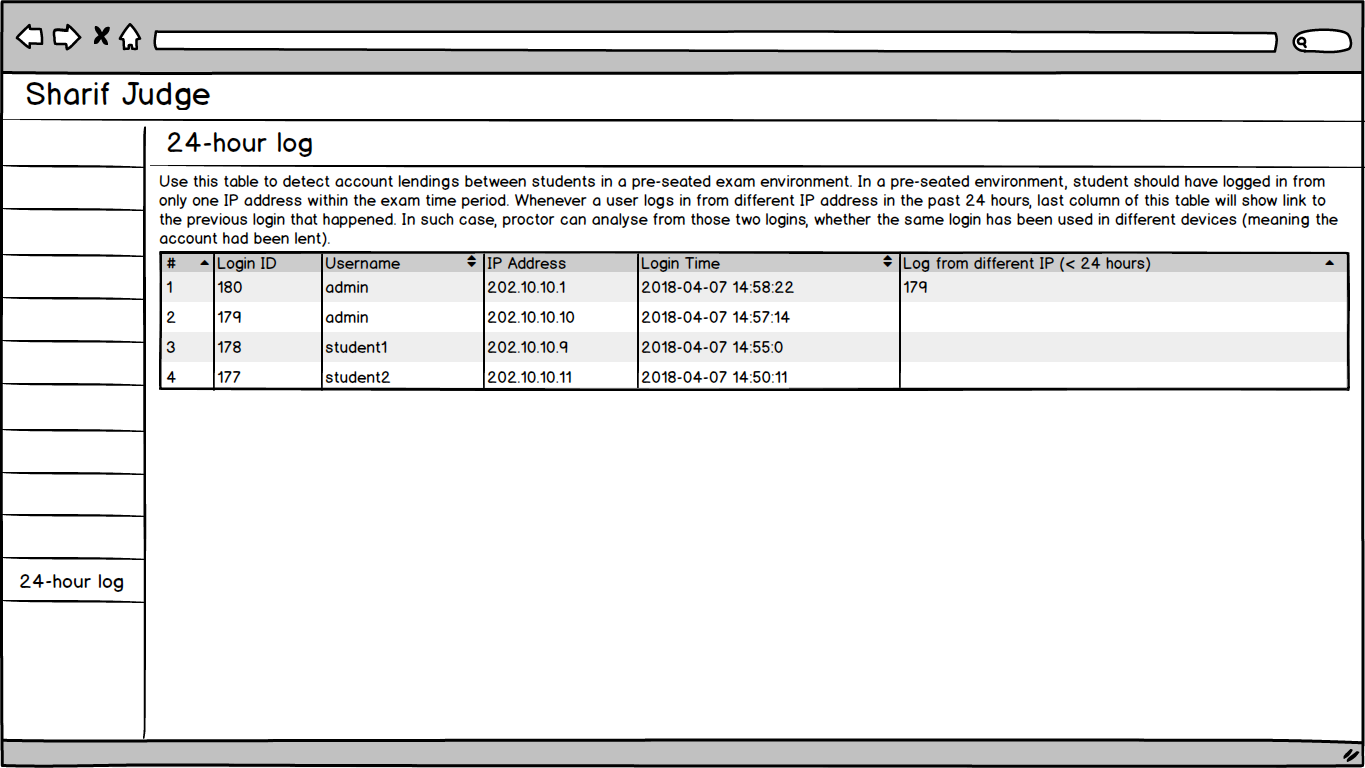
\includegraphics[width=1.0\textwidth]{mockuplogs}  
		\caption[Rancangan tampilan halaman logs]{Rancangan tampilan halaman logs} 
		\label{fig:mockuplogs} 
	\end{figure}

	\item Controller \\
	Controller untuk halaman logs akan bernama Logs.php. Berikut adalah perincian fungsi yang terdapat dalam rancangan model Logs\_model.php.
	\begin{table}[H]
		\caption{Perincian fungsi index}
		\begin{tabular}{|c|p{11cm}|}
			\hline
			Nama Method 	& 	index 	\\
			\hline
			Parameter Input & - \\
			\hline
			Parameter Output &  - \\
			\hline
			Tabel yang berhubungan & shj\_logins \\
			\hline
			Deskripsi	& Proses untuk memuat seluruh entri logs pada halaman Logs.twig	 \\
			\hline
			Algoritma	& \begin{itemize}
				\item memuat data logs menggunakan fungsi get\_all\_logs dari model Logs\_model.php
				\item memproses data untuk tampilan Logs.twig
			\end{itemize} \\
			\hline
		\end{tabular}
	\end{table}
\end{enumerate}
